\section{Wzorce projektowe (1) - konstrukcyjne}
Wzorce kreacyjne pozwalają na tworzenie obiektów w sposób zwiększający elastyczność. Zamiast tworzyć obiekty w wielu miejscach w programie, zadaniem konstrukcji nowych instancji można obciążyć osobne klasy. Użycie słowa kluczowego \texttt{new} narusza omawianą wcześniej zasadę odwracania zależności, powodując trudności z testowaniem kodu i zmniejszając jego elastyczność. 
%\url{https://softwareengineering.stackexchange.com/questions/365119/is-using-new-in-the-constructor-always-bad}

\subsection{Fabryka abstrakcyjna (ang. abstract factory)}\label{sec/lab2/abstractFactory}
Fabryka abstrakcyjna jest wzorcem projektowym, który przenosi proces tworzenia obiektów (często ze sobą w~jakiś sposób powiązanych) do osobnej klasy implementującej interfejs zawierający metody tworzące dane obiekty. Tworzone przez fabryki instancje powinny posiadać zgodne interfejsy.

Klient może posiadać konstruktor, który jako parametr przyjmie obiekt implementujący interfejs abstrakcyjny. Wewnątrz konstruktora klient wywołując odpowiednie metody może tworzyć konkretne obiekty bez znajomości ich szczegółowej implementacji. Przekazując inny obiekt fabryki abstrakcyjnej możliwa jest łatwa zmiana wykorzystywanych przez klienta obiektów.

Jako przykład można wyobrazić sobie aplikację wykorzystującą interfejs graficzny, która przyjmuje jako argument obiekty fabryki implementujące interfejs \texttt{IGuiFactory}. Interfejs ten mógłby definiować metody tworzenia poszczególnych elementów graficznych np. \texttt{CreateButton()}, \texttt{CreateListBox()}, \texttt{CreateProgressBar()} itp. Następnie w zależności od systemu operacyjnego można by stworzyć obiekty fabryk \texttt{WindowsFactory} oraz \texttt{UnixFactory}, oba implementujące określony wcześniej interfejs. Aplikacja posiadające logikę rysująca okno użytkownika nie musi w takim przypadku nawet wiedzieć z jakim systemem ma do czynienia, jest od niego niezależna. Może wywoływać metody tworzące kontrolki UI za pomocą abstrakcyjnego interfejsu \texttt{IGuiFactory}. Wybór konkretnej fabryki mógłby być określany w momencie uruchamiania się aplikacji.

\begin{figure}[hbt!]
	\centering
	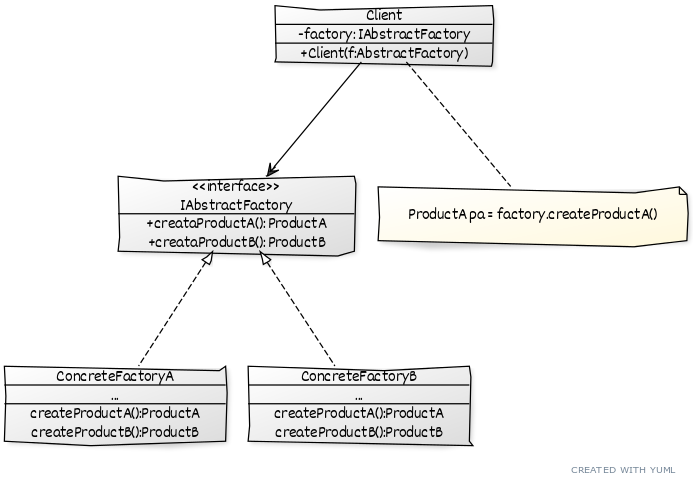
\includegraphics[width=0.9\linewidth]{images/AbstractFactoryUml}
	\caption{Diagram UML wzorca Fabryka Abstrakcyjna.}
	\label{lab2/fig/AbstractFactoryUml}
\end{figure}
%[Client]->[IAbstractFactory]
%[Client]-[note: ProductA pa = factory.CreateProductA(){bg:cornsilk}]
%[IAbstractFactory]^-.-[ConcreteFactoryA]
%[IAbstractFactory]^-.-[ConcreteFactoryB]
%
%[≪interface≫;IAbstractFactory|+CreataProductA(): ProductA;+CreataProductB(): ProductB;]
%[Client|-factory: IAbstractFactory|+Client(f:AbstractFactory);]
%[ConcreteFactoryA|...|CreateProductA():ProductA;CreateProductB():ProductB]
%[ConcreteFactoryB|...|CreateProductA():ProductA;CreateProductB():ProductB]

%//TODO: https://github.com/ninject/Ninject.Extensions.Factory vs https://docs.autofac.org/en/latest/advanced/delegate-factories.html

\subsubsection{Zadanie 1}

Utwórz nowy projekt aplikacji konsolowej .NET 5.0. W osobnych plikach stwórz trzy interfejsy: \texttt{IButton}, \texttt{ICheckbox} oraz \texttt{IGuiFactory}. Pierwsze dwa niech posiadają jedną metodę \texttt{void Draw()}, natomiast interfejs fabryki \texttt{IGuiFactory} dwie metody:\texttt{IButton CreateButton()} oraz \texttt{ICheckbox CreateCheckBox()}.

Umieść w~projekcie dwa foldery \texttt{Macintosh} oraz \texttt{Windows}. Wewnątrz tych folderów dodaj implementacje stworzonych przed chwilą interfejsów. Wszystkie metody \texttt{Draw} zaimplementuj tak, aby wypisywały na ekranie konsoli komunikat symulujący, że kontrolki zostały narysowane np.:
\begin{lstlisting}
internal class MacButton : IButton
{
	public void Draw() => Console.WriteLine("Macintosh button has been drawn");
}
\end{lstlisting}

%Tip: Ustawiając kursor na nazwę interfejsu i klikając Alt+Enter możesz uruchomić narzędzie refaktoryzacyjne i wybrać opcję \texttt{Implement interface}. Visual Studio automatycznie doda do klasy metody wymagające implementacji.

Po napisaniu analogicznych metod dla pozostałych kontrolek, utwórz po jednej klasie fabryki w~każdym z~folderów. Klasa fabryki powinna zwracać instancję klasy odpowiadającej danej kontrolce np.:
\begin{lstlisting}
public class MacFactory : IGuiFactory
{
	public IButton CreateButton() => new MacButton();
	public ICheckbox CreateCheckBox() => new MacCheckbox();
}
\end{lstlisting}

Teraz w katalogu głównym utwórz klasę \texttt{UserInterface}, która będzie posiadała prywatne pole typu \texttt{IGuiFactory}. W~konstruktorze przypisz przekazywany do wnętrza klasy obiekt do utworzonego przed chwilą prywatnego pola. Napisz metodę \texttt{DrawWindow}, w której pobierzesz z~fabryki instancje klas implementujących \texttt{IButton} oraz \texttt{ICheckbox} i wywołasz metodę \texttt{Draw} dla każdego z~nich.

W metodzie \texttt{Main} sprawdź działanie wzorca fabryki abstrakcyjnej:
\begin{lstlisting}
class Program
{
	static void Main(string[] args)
	{
		// Based on configuration file one can choose the specific factory over another one
		var factoryA = new MacFactory();
		var factoryB = new WinFactory();
		
		var uiA = new UserInterface(factoryA);
		uiA.DrawWindow();
		
		var uiB = new UserInterface(factoryB);
		uiB.DrawWindow();
	}
}
\end{lstlisting}

\subsubsection{Inne wzorce fabryk}
%https://refactoring.guru/design-patterns/factory-comparison
Fabryka jest ogólnym terminem, który jest używany w stosunku do metod i klas, które tworzą obiekty. Podczas laboratoriów został omówiony wzorzec fabryki abstrakcyjnej, który służy do tworzenia całych rodzin podobnych albo powiązanych ze sobą obiektów bez precyzowania konkretnych klas. Jeśli jednak program nie wymaga tworzenia takich rodzin najprawdopodobniej fabryka abstrakcyjna nie jest konieczna. 

Inną prostą fabryką może być klasa, która posiada metodę wytwórczą, z wyrażeniem \texttt{switch-case} które analizuje przekazywany do niej parametr i tworzy odpowiednią instancję konkretnej klasy. Często jest to pojedyncza metoda w pojedynczej klasie. Z czasem kiedy liczba tworzonych obiektów rośnie może ona się przekształcić z metodę fabrykującą. 
%\begin{lstlisting}
%class UserFactory {
%	public static function create($type) {
%		switch ($type) {
%			case 'user': return new User();
%			case 'customer': return new Customer();
%			case 'admin': return new Admin();
%			default:
%			throw new Exception('Wrong user type passed.');
%		}
%	}
%}
%\end{lstlisting}

Metoda fabrykująca udostępnia interfejs do tworzenia obiektów, ale pozwala klasom pochodnym zmienić typ tworzonego obiektu. W klasie bazowej umieszczona jest pewna funkcjonalność, do klas pochodnych jest przeniesiony jedynie proces tworzenia obiektów. Jest to szczególny przypadek metody szablonowej.
%\begin{lstlisting}
%abstract class Department {
%	public abstract function createEmployee($id);
%	
%	public function fire($id) {
%		$employee = $this->createEmployee($id);
%		$employee->paySalary();
%		$employee->dismiss();
%	}
%}
%
%class ITDepartment extends Department {
%	public function createEmployee($id) {
%		return new Programmer($id);
%	}
%}
%
%class AccountingDepartment extends Department {
%	public function createEmployee($id) {
%		return new Accountant($id);
%	}
%}	
%\end{lstlisting}

\subsection{Budowniczny (ang. builder)}\label{lab2/sec/builderPattern}
Budowniczy jest wzorcem, który może być wykorzystany do tworzenia złożonego obiektu krok po kroku. Czasami istnieje pokusa stworzenia konstruktora przyjmującego dużą liczbę argumentów. Może tak się zdarzyć jeśli klasa korzysta z~wielu zależności albo niektóre jej cechy mogą być parametryzowane. Część z tych argumentów może dodatkowo być opcjonalna. Budowniczy przenosi proces tworzenia takiej instancji do osobnego obiektu. 

Czynności wywoływania poszczególnych metod można przenieść do obiektu kierownika (ang. director), który będzie przyjmował jako argument konstruktora obiekt budowniczego i wywoływał metody interfejsu \texttt{IBuilder}. Obiekt kierownika jest opcjonalny, klient może samemu tworzyć instancję budowanego typu. 

Konkretni budowniczowie powinni dostarczyć swoje własne metody zwracania wyników procesu budowania obiektu. Różni budowniczowie mogą zwracać zupełnie inne typy dlatego tego procesu często nie da się umieścić w interfejsie \texttt{IBuilder} (przynajmniej w przypadku języków programowania, które są silnie typowane). 
 
Dodatkowo należy wspomnieć, że wzorzec budowniczy często wykorzystuje tzw. Płynny Interfejs (ang. Fluent Interface). Polega on na łańcuchowym połączeniu metod. Pozwala na zwiększenie czytelności kodu. Kaskadowe połączenie metod realizuje się zwracając w metodzie instancję własnej klasy za pomocą słowa kluczowego \texttt{this}. Z przykładem użycia tego mechanizmu można się spotkać w zapytaniach LINQ\ref{lab2/lst/fluentInterfaceLinq}, gdzie zamiast wywoływać kolejne metody progresywnie (w kolejnych wierszach), można je wywoływać kaskadowo po symbolu kropki. 

\begin{lstlisting}[caption={Wykorzystanie płynnych interfejsów w zapytania LINQ}, label={lab2/lst/fluentInterfaceLinq}]
var translations = new Dictionary<string, string>
{
	{"cat", "chat"},
	{"dog", "chien"},
	{"fish", "poisson"},
	{"bird", "oiseau"}
};

// Find translations for English words containing the letter "a",
// sorted by length and displayed in uppercase
IEnumerable<string> query = translations
.Where(t => t.Key.Contains("a"))
.OrderBy(t => t.Value.Length)
.Select(t => t.Value.ToUpper());

// The same query constructed progressively:
var filtered = translations.Where(t => t.Key.Contains("a"));
var sorted  = filtered.OrderBy(t => t.Value.Length);
var finalQuery = sorted.Select(t => t.Value.ToUpper());
\end{lstlisting}

W przeciwieństwie do wzorca fabryki abstrakcyjnej, która tworzy obiekty w~jednym kroku, budowniczy tworzy jeden złożony obiekt krok po kroku.

\subsubsection{Zadanie 2}

Utwórz projekt .NET 5.0. Dodaj do niego klasę \texttt{Car} i dodaj do niej właściwości ze słowem kluczowym \texttt{init}\footnote{Słowo kluczowe \texttt{init} pojawiło się w C\# 9.0 i~stanowi ułatwienie w tworzeniu obiektów niemutowalnych (niezmiennych). Wcześniej konieczne było wykorzystywanie słowa kluczowego \texttt{readonly} i tworzenie obszernych konstruktorów.}\ref{lab2/lst/immutableProperties}. 

% OPOWIEDZIEĆ O REKORDACH
%Ponieważ w przypadku chęci utworzenia nowego obiektu niemutowalnego, który będzie posiadał inne wartości tylko kilku właściwości konieczne jest tworzenie nowego obiektu i ponowne przypisanie za pomoc listy inicjalizacji wszystkich właściwości pojawiły się w C\# również rekordy. Wykorzystując rekordy można przy przypisywaniu rekordu do innego rekordu użyć słowa kluczowego \texttt{with} i zmienić tylko tę jedną właściwość na której nam zależy, reszta zostanie automatycznie przepisana. Dodatkowo w przypadku rekordów porównywanie dwóch obiektów przebiega pole po polu. Kompilator automatycznie tworzy konstruktor kopiujący. Rekord wraz z~konstruktorem oraz destruktorem tworzy się za pomocą poniższego zapisu:
%\begin{lstlisting}
%	public record Friend(string FirstName,string MiddleName, string LastName);
%\end{lstlisting}
%Obiekt typu \texttt{Friend} będzie posiadał właściwości takie jak argumenty rekordu.
%Przykład stosowanie rekordów:
%\begin{lstlisting}
%	using System;
%	namespace RecordsVS
%	{
%		public record Friend
%		{
%			public string FirstName { get; init; }
%			public string MiddleName { get; init; }   
%			public string LastName { get; init; }        
%		}
%		public record SuperFriend : Friend
%		{
%			public bool IsBestFriend { get; init; }
%		}
%		class Program
%		{
%			static void Main(string[] args)
%			{
%				var friendA = new Friend()
%				{
%					FirstName = "Chandler",
%					MiddleName = "Miruel",
%					LastName = "Bing"
%				};
%				var friendB = friendA with {LastName = "Geller"};
%				var friendC = friendB;
%				var superFriendA = new SuperFriend()
%				{
%					FirstName = "Ross",
%					LastName = "Geller",
%					IsBestFriend = true,
%				};
%				Friend friendD = superFriendA;
%				Console.WriteLine(friendB); //Friend { FirstName = Chandler, MiddleName = Miruel, LastName = Geller }
%				Console.WriteLine(friendA == friendB); //not equal
%				Console.WriteLine(friendB == friendC); //equal
%				
%				System.Console.WriteLine(friendD == superFriendA);//true
%			}
%		}
%	}
%\end{lstlisting}



\begin{lstlisting}[caption={Inicjalizacja obiektu klasy \texttt{Car} ze niemutowalnymi właściwościami}, label={lab2/lst/immutableProperties}]
public string Manual { get; init;}
public string Engine { get; init; }
public string Seats { get; init; }
public string TripComputer { get; init; }
public string Gps { get; init; }
\end{lstlisting}


Zdefiniuj w klasie \texttt{Car} konstruktor z modyfikatorem dostępu \texttt{private}:
\begin{lstlisting}
private Car() { }
\end{lstlisting}

W osobnym pliku utwórz interfejs \texttt{ICarBuilder}, który będzie posiadał następujące metody zwracające \texttt{void}:
\begin{itemize}
	\item Reset(),
	\item SetEngine(),
	\item SetSeats(),
	\item SetTripComputer(),
	\item SetGps().
\end{itemize}

Wewnątrz klasy \texttt{Car}, zdefiniuj klasę \texttt{CarBuilder} implementującą interfejs \texttt{ICarBuilder}. Zwróć uwagę, że klasa ta ma dostęp do prywatnych składowych klas (w tym konstruktora). Utworzenie instancji tej klasy będzie możliwe jedynie przez klasę budowniczego. W~\texttt{CarBuilder} utwórz prywatne pola typu \texttt{string}: \texttt{seats}, \texttt{engine}, \texttt{tripComputer} oraz \texttt{gps}.

Zaimplementuj interfejs \texttt{ICarBuilder}. W każdej metodzie ustawiającej dany fragment samochodu, przypisz jakiś łańcuch znaków pozwalający na późniejszą identyfikację np.:
\begin{lstlisting}
public class CarBuilder : ICarBuilder
{
	private string seats;
	//...
	
	public void SetSeats() => this.seats = "Four fancy seats";
	//...		
}
\end{lstlisting}

Do klasy \texttt{CarBuilder} dodaj metodę \texttt{Build} zwracającą typ \texttt{Car}. Utwórz w niej instancję klasy \texttt{Car}, przypisz do jej właściwości ustawione wcześniej wartości prywatnych pól np.:
\begin{lstlisting}
public Car Build()
{
	var car = new Car()
	{
		Engine = this.engine,
		//...
	};
	
	//...
}
\end{lstlisting}

W metodzie \texttt{Main} utwórz korzystając z budowniczego instancję klasy \texttt{Car}. Aby to zrobić stwórz obiekt \texttt{CarBuilder}, następnie wywołaj metody ustawiające poszczególne właściwości (nie jest konieczne wywoływanie ich wszystkich) i utwórz obiekt za pomocą metody \texttt{Build}. Sprawdź czy utworzona instancja typu \texttt{Car} zawiera prawidłowe wartości odpowiednich właściwości tej klasy.  Możesz to zrobić wypisując je na ekranie konsoli. Ewentualnie można przeciążyć metodę \texttt{ToString} tak, aby zwracała łańcuch znaków zawierający te informacje.

Utwórz klasę kierownika \texttt{Director}. Niech posiada ona prywatne pole typu \texttt{ICarBuilder} oraz właściwość \texttt{set}:
\begin{lstlisting}
private ICarBuilder _builder;
public ICarBuilder Builder { set { _builder = value; } }
\end{lstlisting}
Dodatkowo umieść w niej dwie metody: \texttt{BuildMinimalViableProduct} oraz \texttt{BuildFullFeaturedProduct}. Obie metody niech zwracają typ \texttt{void}. W pierwszej wywołaj dwie z dostępnych metod tworzenia obiektu przez budowniczego, w drugim wszystkie.
% Viable - wykonalny, realny

Z poziomu metody \texttt{Main} utwórz obiekt \texttt{CarBuilder} oraz \texttt{Director}. Przypisz kierownikowi obiekt budowniczego. Następnie wywołaj jedną z dostępnych metod kierownika. Na koniec pobierz ,,zbudowany'' obiekt za pomocą metody \texttt{Build} klasy \texttt{CarBuilder}. Sprawdź utworzone elementy obiektu \texttt{Car}.

\subsubsection{Zadanie 3}
Wewnątrz klasy \texttt{Car} utwórz drugiego budowniczego. Tym razem do implementacji wykorzystaj tzw. Płynne Interfejsy. Jedyną różnicą względem poprzedniej implementacji będzie fakt, że tym razem metody ustawiające wartości prywatnym polom (te metody, który ,,budują'' obiekt), będą zwracały instancję klasy budowniczego. Konieczne jest skorzystanie ze słowa kluczowego \texttt{this} zwracającego instancję kasy:
\begin{lstlisting}
public CarBuilderFluent SetSeats()
{
	this.seats = "Four fancy seats";
	return this;
}
\end{lstlisting}

Sprawdź działanie drugiej wersji wzorca projektowego Budowniczy. Tym razem kolejne metody można wywoływać z wykorzystaniem symbolu kropki.
\begin{lstlisting}
// Builder with a fluent interface
var builderFluent = new Car.CarBuilderFluent();
var carFluent = builderFluent.SetEngine()
	.SetGPS()
	.SetSeats()
	.SetTripComputer()
	.Build();
\end{lstlisting}